\documentclass[a4paper,11pt]{report}

\usepackage{amsmath,amssymb}
\usepackage{fullpage}
\usepackage{graphicx}
\usepackage[cache=false]{minted}

\usepackage{bussproofs}
\usepackage{mathpartir}
\usepackage{prooftrees}
\usepackage{color}

\usepackage{tikz}
\usetikzlibrary{automata,positioning}

\newcommand*\circled[1]{\tikz[baseline=(char.base)]{
    \node[shape=circle,draw,inner sep=2pt] (char) {#1};}}

\makeatletter
\pgfmathdeclarefunction{alpha}{1}{%
  \pgfmathint@{#1}%
  \edef\pgfmathresult{\pgffor@alpha{\pgfmathresult}}%
}

\newcommand*{\until}{U}
\newcommand*{\disj}{\ ,\ }
\newcommand*{\A}{\square}  % Always
\newcommand*{\D}{\diamondsuit} % eventually

\newcommand*{\Pq}{(\top,\bot)}
\newcommand*{\pQ}{(\bot,\top)}
\newcommand*{\PQ}{(\top,\top)}
\newcommand*{\pq}{(\bot,\bot)}

\usemintedstyle{tango}

\newminted[promelacode]{C}{
  frame=single,
  framesep=6pt,
  breaklines=true,
  fontsize=\scriptsize
}

\newmintinline[promelainline]{C}{breaklines=true,fontsize=\small}

\newmintedfile{c}{frame=single, framesep=6pt, breaklines=true,fontsize=\scriptsize}
\newcommand{\ex}[3]{\cfile[firstline=#1,lastline=#2]{ex#3.pml}}

% tikz
\usepackage{tikz}
\usetikzlibrary{snakes}

\author{Sylvain Julmy}
\date{\today}

\setlength{\parindent}{0pt}
\setlength{\parskip}{2.5pt}

\begin{document}

\begin{center}
  \Large{
    Verification of Cyber-Physical System\\
    Fall 2017
  }
  
  \noindent\makebox[\linewidth]{\rule{\linewidth}{0.4pt}}
  Exercice Sheet 8

  \vspace*{1.4cm}

  Author : Sylvain Julmy
  \noindent\makebox[\linewidth]{\rule{\linewidth}{0.4pt}}

  \begin{flushleft}
    Professor : Ultes-Nitsche Ulrich
    
    Assistant : Prisca Dotti
  \end{flushleft}

  \noindent\makebox[\linewidth]{\rule{\textwidth}{1pt}}
\end{center}

\section*{Sender}

The idea to implement the sender, is to create a generic sender no matter how
many bit we send. We just indicates the bit to send and the automaton will
switch the signal value w.r.t. the current bit to send.

The figures \ref{fig:sender} illustrate the times automaton design for the
sender. Basically, the automaton wait in the central state for
$\frac{\Delta^T}{2}$ and will move to the next state depending on the current
signal value and the next bit to send.

\begin{figure}[h]
  \centering
  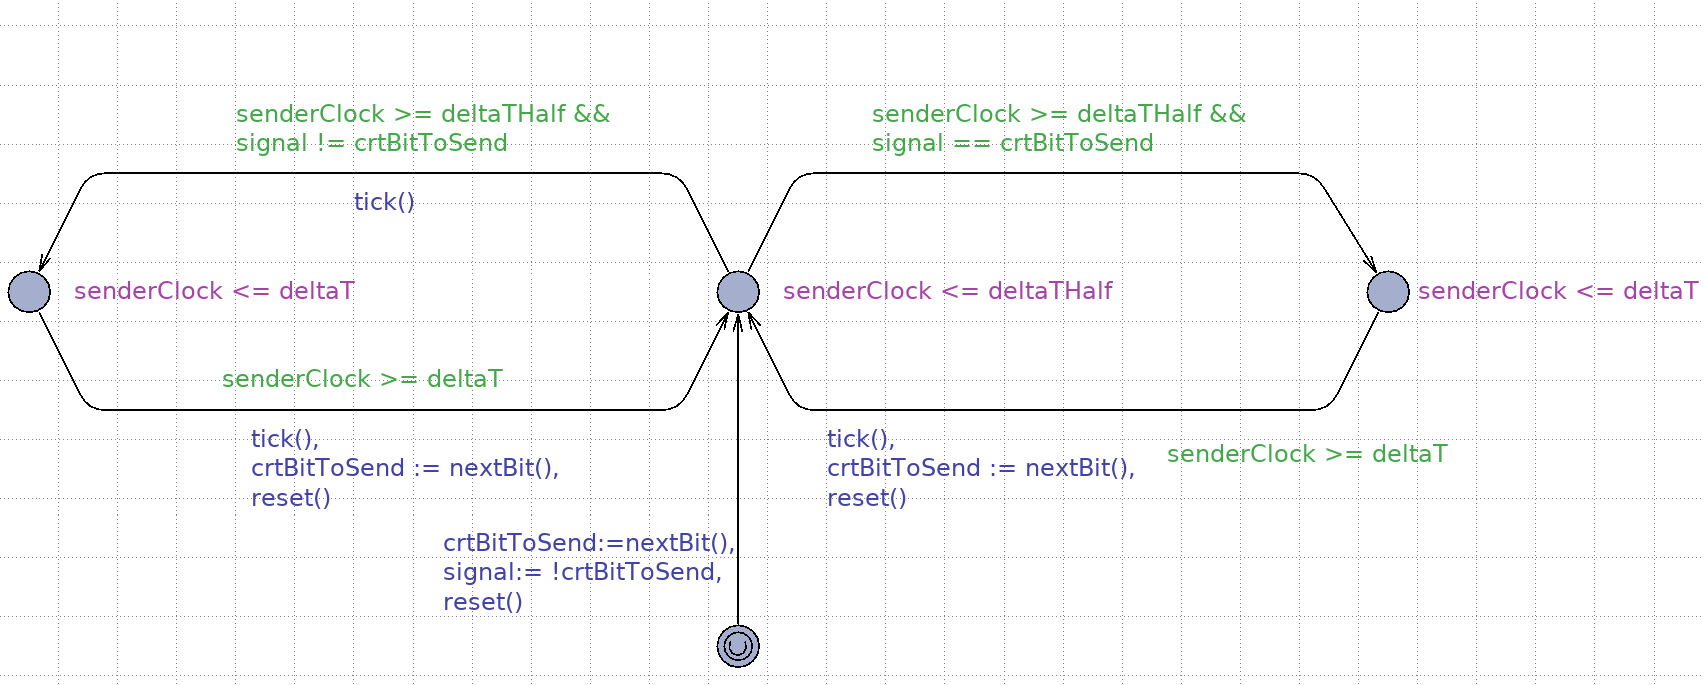
\includegraphics[width=0.9\textwidth]{figures/sender}
  \caption{\label{fig:sender} Sender automaton design}
\end{figure}

If the signal value is the same as the next bit to send, we have to tick
before moving to either the left or right state.

Then both state do the same thing by ticking the signal, reseting the clock and
computing the next bit to send.

The following listing is the implementation of the various function use for the
sender automaton.

\begin{promelacode}
const int deltaT = 10000;
const int deltaTHalf = deltaT/2;
clock senderClock;
int bitCount=0;

bool preamble[64] = {
    1,0,1,0,1,0,1,0,1,0,1,0,1,0,1,0,1,0,
    1,0,1,0,1,0,1,0,1,0,1,0,1,0,1,0,1,0,
    1,0,1,0,1,0,1,0,1,0,1,0,1,0,1,0,1,0,
    1,0,1,0,1,0,1,0,1,1};

bool data[64] = {
    1,1,1,0,0,0,1,0,1,1,1,0,1,0,1,1,0,0,
    1,0,1,0,0,0,1,1,1,1,1,1,1,1,0,0,0,0,
    1,0,0,0,0,0,1,0,0,0,0,0,0,0,1,0,1,0,
    1,1,0,0,0,0,0,0,1,1};

bool crtBitToSend;

void reset()
{
    senderClock := 0;
}

// return the next bit to send
bool nextBit()
{
    int itr = bitCount % 64;
    if(bitCount > 127) return 1;
    if(bitCount++ < 64) {
        return preamble[itr];
    } else {
        return data[itr];
    }
}

void tick()
{
    signal := !signal;
}
\end{promelacode}

\newpage

\section*{Receiver}

The receiver is not finish yet, but the idea is the following :

\begin{itemize}
\item Initialize $\Delta^t$ to a random value,not equals to $0$
\item During the preamble period, we adjust $\Delta^T$ with a specific learning
  rate (like $0.1$)
\item Detect the double $1$ bit which indicates the end of the preamble
\item Receive the data
\end{itemize}

\begin{figure}[ht]
  \centering
  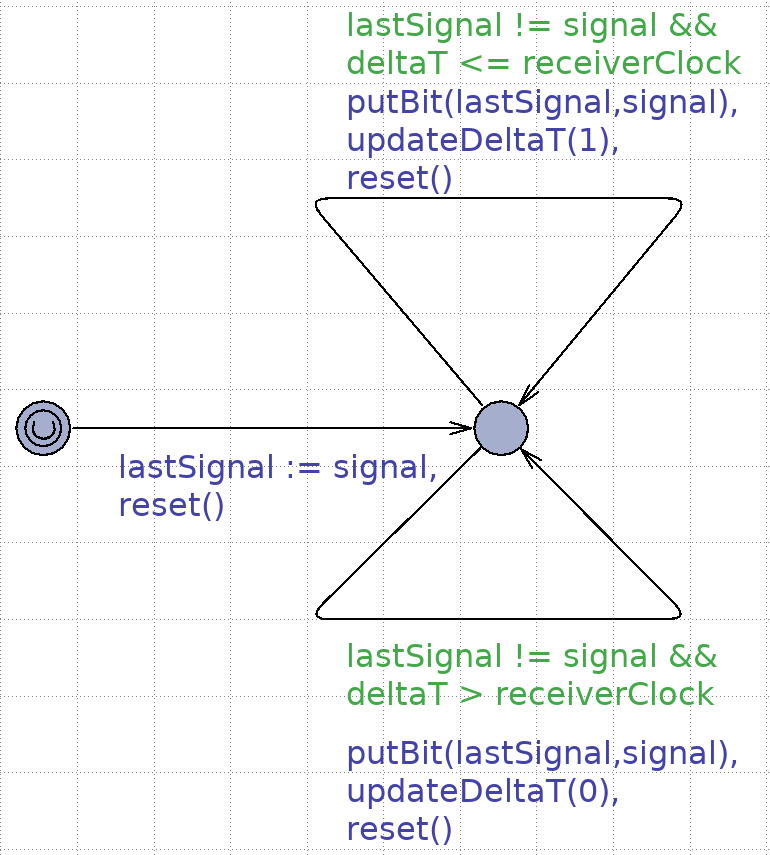
\includegraphics[width=0.7\textwidth]{figures/receiver}
  \caption{\label{fig:receiver} Receiver automaton design}
\end{figure}

The following listing is the implementation of the various function and
variables use by the sender.

\newpage

\begin{promelacode}
clock receiverClock;

// array to receive the data and compare at the end
bool data[64] = {
    0,0,0,0,0,0,0,0,0,0,0,0,0,0,0,0,0,0,0,
    0,0,0,0,0,0,0,0,0,0,0,0,0,0,0,0,0,0,0,
    0,0,0,0,0,0,0,0,0,0,0,0,0,0,0,0,0,0,0,
    0,0,0,0,0,0,0};

bool preamble[64] = {
    0,0,0,0,0,0,0,0,0,0,0,0,0,0,0,0,0,0,0,
    0,0,0,0,0,0,0,0,0,0,0,0,0,0,0,0,0,0,0,
    0,0,0,0,0,0,0,0,0,0,0,0,0,0,0,0,0,0,0,
    0,0,0,0,0,0,0};

int crtBitToReceiveIndex = 0;
double deltaT = 100.0;

// learning rate
double lr = 0.1;

bool lastSignal;

void reset()
{
    receiverClock := 0;
}

int bitCount = 0;

// PRE lastSignal != signal
void putBit(bool lastSignal,bool signal) {
    bool bit;
    int itr = bitCount % 64;

    if(lastSignal && !signal) {
        bit = 1;
    } else {
        bit = 0;
    }

    if(bitCount < 64) {
        preamble[itr] = bit;
    }
    else {
        data[itr] = bit;
    }
    bitCount++;
}

// update deltaT during the receive of the preamble
void updateDeltaT(bool direction) {
    if(direction) { // need to decrease deltaT
        deltaT := deltaT - deltaT * lr;
    }
    else { // otherwise deltaT is to small
        deltaT := deltaT + deltaT * lr;
    }
}
\end{promelacode}

\end{document}
